\ifthenelse{\equal{\doclanguage}{Italian}}
{\chapter{methodology}}
{\chapter{Metodologia e Tecnologie}}
\label{sec:methodology}

La GDS offre oggi un ampio catalogo di algoritmi per la generazione di graph embedding, ciascuno fondato su architetture profondamente diverse. Questa varietà, pur costituendo una ricchezza dal punto di vista teorico, pone un problema pratico immediato a chi intende applicare la GDS a un dominio reale: la scelta dell'algoritmo non è banale, poichè ogni modello elabora le informazioni contenute nel KG attraverso le funzioni di aggregazione  e produce rappresentazioni vettoriali molto differenti. Di conseguenza, la qualità degli embedding ottenuti, e la loro utilità per un task predittivo specifico, dipende in modo diretto da questa scelta architetturale.

Alla luce di queste considerazioni teoriche, il presente studio si propone di affrontare il problema della selezione algoritmica attraverso una rigorosa valutazione empirica. L'obiettivo centrale consiste nel confrontare diversi approcci di generazione di graph embedding per valutarne oggettivamente la qualità sulle strutture relazionali tipiche di un KG biomedico. Il task di \textit{link prediction} viene adottato come strumento di misurazione direttaa: la capacità di un modello di prevedere connessioni non osservate tra entità del grafo riflette direttamente quanto gli embedding prodotti abbiano saputo catturare le proprietà topologiche e semantiche della rete sottostante. In ambito farmacologico, questo corrisponde all'identificazione di relazioni terapeutiche latenti tra entità biologiche, un obiettivo con implicazioni dirette nel dominio del drug repurposing.

\section{Motivazione della scelta degli algoritmi}
La metodologia sperimentale adottata in questo studio si discosta dai tradizionali approcci che si limitano a misurare l'accuratezza predittiva. Al contrario, il presente lavoro propone un'indagine empirica strutturata su un duplice livello di analisi volto a coniugare la valutazione prestazionale dei modelli di apprendimento automatico con l'analisi degli algoritmi di generazione di graph embeddings sottostanti. 

L'ipotesi fondante di questa metodologia è che, in scenari applicativi reali come il \textit{drug repurposing}, il valore di una pipeline non dipenda esclusivamente dalla sua capacità di generalizzazione statistica, ma anche dalla sua sostenibilità in scenari caratterizzati da un grande volume. Per condurre una valutazione esaustiva e tracciare un profilo completo delle soluzioni analizzate, l'indagine si sviluppa lungo tre direttrici principali:

\begin{itemize}
    \item \textbf{Valutazione Algoritmica}: analisi della qualità degli \textit{embedding} generati. Il confronto tra approcci induttivi, trasduttivi ed eterogenei ha lo scopo di determinare quale architettura modelli in modo più efficace la struttura e la semantica del grafo biomedico. Le prestazioni vengono misurate in base a tre parametri: l'accuratezza predittiva sulla \textit{link prediction} (calcolata tramite la metrica AUC-ROC), il costo computazionale (tempi di addestramento e velocità di convergenza) e la gestione nativa dell'eterogeneità dei nodi.
    
    \item \textbf{Valutazione Infrastrutturale}: misurazione delle prestazioni del database distribuito in fase di lettura. Poiché i dati devono essere trasferiti dal layer di \textit{storage} alla pipeline di \textit{Machine Learning}, si analizza il tempo di estrazione sequenziale del sottografo al variare del numero di nodi attivi nel cluster. L'obiettivo è quantificare l'impatto dell'\textit{overhead} di rete e verificare se la scalabilità orizzontale produca un reale aumento del \textit{throughput} o se introduca colli di bottiglia.
    
    \item \textbf{Validazione Statistica e Riproducibilità}: per garantire che i risultati non siano alterati dall'inizializzazione casuale dei pesi o da fluttuazioni statistiche, ogni esperimento viene eseguito su cinque \textit{run} indipendenti. 
\end{itemize}

L'integrazione di queste tre direttrici consente non solo di decretare quale algoritmo performi meglio in termini assoluti, ma di definire il miglior \textit{trade-off} tra complessità computazionale, accuratezza predittiva e agilità infrastrutturale.
s
La selezione di GraphSAGE, TransE e HashGNN permette di mettere a confronto tre metodi di calcolo profondamente diversi, con l'obiettivo di capire quale di queste strutture sia più efficace nel produrre embedding di alta qualità, in particolare:
\begin{itemize}
    \item \textbf{GraphSAGE} \cite{hamilton2017inductive} è stato scelto per valutare l'efficacia di un approccio induttivo, verificando quanto la semplice aggregazione omogenea del vicinato locale sia informativa per prevedere nuovi collegamenti;
    \item \textbf{TransE} \cite{bordes2013translating} offre invece una prospettiva opposta e trasduttiva, permettendo di misurare quanto la modellazione puramente geometrica delle relazioni incida sull'accuratezza e fornendo un solido termine di paragone per l'efficienza computazionale;
    \item  \textbf{HashGNN} \cite{neo4j_hashgnn}, infine, è stato inserito per colmare i limiti di GraphSAGE nella gestione dell'eterogeneità, consentendo di verificare empiricamente se mantenere spazi vettoriali separati per entità differenti produca un reale vantaggio predittivo.    
\end{itemize}



\section{Architettura dell'esperimento}

A partire dal KG di riferimento, viene estratto un sottografo tematico che definisce il perimetro sperimentale, selezionando i tipi di nodo e il tipo di relazione di interesse. Su tale sottografo vengono applicati i tre algoritmi, ciascuno dei quali produce embedding vettoriali per i nodi della rete. La qualità di queste rappresentazioni latenti viene valutata tramite un \textbf{classificatore binario} addestrato sul task di \textit{link prediction}: data una coppia di nodi, il modello inferisce la probabilità che tra loro esista una connessione reale, producendo uno score $p \in [0, 1]$. 

Questa formulazione permette di misurare direttamente quanto ciascun approccio riesca a catturare la struttura relazionale della rete e a generalizzare su connessioni non osservate durante il training.

In parallelo, l'analisi si estende al livello infrastrutturale, misurando l'impatto della scalabilità orizzontale del sistema di storage distribuito sui tempi di estrazione dei dati verso la pipeline di apprendimento. Questa dimensione è spesso trascurata nella letteratura in favore della sola accuratezza predittiva, ma risulta critica in scenari di elaborazione reale: un overhead di comunicazione e coordinamento eccessivo tra i nodi del cluster può trasformarsi nel principale collo di bottiglia dell'intera pipeline, annullando i benefici computazionali dell'architettura distribuita. Quantificare empiricamente questo impatto, variando il numero di nodi attivi nel cluster, costituisce uno degli obiettivi originali di questo lavoro.

Per assicurare l'affidabilità statistica del confronto, l'intero ciclo di esperimenti viene ripetuto su cinque esecuzioni indipendenti con inizializzazioni diverse, permettendo di distinguere risultati sistematici da fluttuazioni casuali legate all'inizializzazione dei pesi.


% LE RISCRIVO SOTTO E I DETTAGLI LI INSERISCO NELL'IMPLEMENTAZIONE, QUI SOLO UN'INFARINATURA

\begin{comment}
\section{Strumenti e tecnologie}
L'implementazione della pipeline sperimentale si basa su strumenti selezionati per la loro complementarità, ciascuno responsabile di una fase specifica del flusso di elaborazione.

\subsection{Neo4j}

Neo4j è un database a grafo \textbf{nativo}: implementa il modello Property Graph fino al livello fisico di memorizzazione, senza strati di astrazione intermedi. I dati vengono archiviati esattamente nella forma in cui vengono modellati, e l'attraversamento della rete avviene tramite puntatori fisici diretti tra nodi e archi, con un costo costante $O(1)$ per ogni passo di traversata indipendentemente dalla dimensione del database. Il linguaggio di interrogazione nativo è \textbf{Cypher}, un linguaggio dichiarativo progettato per esprimere pattern strutturali su grafi in modo intuitivo e orientato alla navigazione di nodi e relazioni. 

\textbf{Neo4j Enterprise} \cite{neo4j_gds} è la versione adottata in questo lavoro, che abilita la configurazione in cluster distribuito con topologia primary-secondary, necessaria per il benchmark infrastrutturale.

\subsection{Libreria Graph Data Science}

La libreria \textbf{Graph Data Science} (GDS) \cite{neo4j_gds} è un'estensione di Neo4j che espone implementazioni parallele di algoritmi analitici su grafi come procedure Cypher. Il meccanismo centrale è la \textbf{graph projection}: prima dell'esecuzione di un algoritmo, il sottografo di interesse viene proiettato in una struttura in memoria separata, denominata \textit{graph catalog}, ottimizzata per il calcolo analitico. Questo separa nettamente il layer transazionale da quello analitico, permettendo l'esecuzione di algoritmi intensivi senza interferire con le operazioni correnti sul database.

\begin{figure}[ht!]
\centering
\resizebox{0.65\textwidth}{!}{
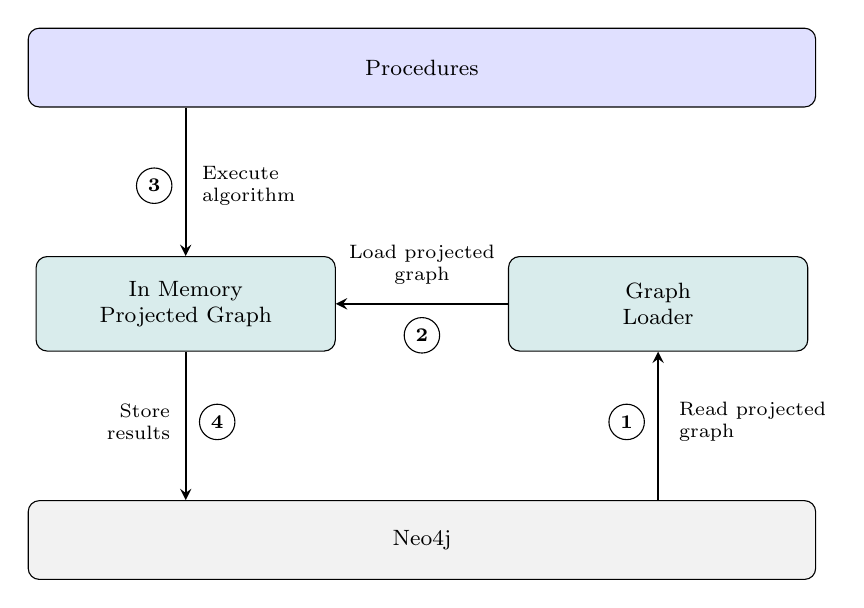
\begin{tikzpicture}[
  box/.style={rectangle, draw, rounded corners, minimum height=1cm,
              font=\footnotesize, align=center},
  wide_box/.style={box, minimum width=10cm},
  node_box/.style={box, minimum width=3.8cm, minimum height=1.2cm},
  arrow/.style={->, thick, >=stealth},
  number/.style={circle, draw, fill=white, inner sep=1.5pt,
                 minimum size=0.45cm, font=\scriptsize\bfseries}
]
  \node[wide_box, fill=blue!12]  (proc)   at (0, 6) {Procedures};
  \node[wide_box, fill=gray!10]  (neo4j)  at (0, 0) {Neo4j};
  \node[node_box, fill=teal!15]  (impg)   at (-3, 3)
    {In Memory\\Projected Graph};
  \node[node_box, fill=teal!15]  (loader) at (3, 3)
    {Graph\\Loader};

  \draw[arrow] (neo4j.north -| loader.south) -- (loader.south);
  \node[align=left, font=\scriptsize] at (4.2, 1.5)
    {Read projected\\graph};
  \node[number] at (2.6, 1.5) {1};

  \draw[arrow] (loader.west) -- (impg.east);
  \node[align=center, font=\scriptsize] at (0, 3.5)
    {Load projected\\graph};
  \node[number] at (0, 2.6) {2};

  \draw[arrow] (proc.south -| impg.north) -- (impg.north);
  \node[align=left, font=\scriptsize] at (-2.2, 4.5)
    {Execute\\algorithm};
  \node[number] at (-3.4, 4.5) {3};

  \draw[arrow] (impg.south) -- (neo4j.north -| impg.south);
  \node[align=right, font=\scriptsize] at (-3.6, 1.5)
    {Store\\results};
  \node[number] at (-2.6, 1.5) {4};
\end{tikzpicture}
}
\caption{Ciclo di vita dell'esecuzione degli algoritmi tramite la libreria Neo4j GDS: il grafo viene proiettato in memoria, l'algoritmo viene eseguito sulla proiezione e i risultati vengono scritti nel database.}
\label{fig:neo4j_gds_architecture}
\end{figure}

\subsection{PyTorch Geometric}
\textbf{PyTorch Geometric} \cite{fey2019fast} è il framework di riferimento per l'implementazione dei tre modelli di Graph Machine Learning. Sviluppato come estensione di PyTorch, fornisce primitive efficienti per la rappresentazione di grafi eterogenei attraverso il formato \texttt{HeteroData}, layer convoluzionali dedicati (come \texttt{SAGEConv}) e utility per la suddivisione del dataset in training, validazione e test, gestendo automaticamente il campionamento dei vicini e il batching su GPU. La sua integrazione nativa con il calcolo tensoriale di PyTorch e il supporto a meccanismi di messaggio personalizzati lo rendono particolarmente adatto per sperimentare con architetture diverse su grafi di larga scala.

\subsection{Docker e Docker Compose}
\textbf{Docker e Docker Compose} sono utilizzati per la containerizzazione dell'ambiente Neo4j su ciascun nodo del cluster. Docker garantisce isolamento delle dipendenze e riproducibilità dell'ambiente di esecuzione, indipendentemente dalla configurazione del sistema operativo sottostante, mentre Docker Compose coordina la definizione e l'avvio dei servizi (Neo4j, eventuali tool di monitoring) tramite un unico file YAML. Questa strategia semplifica il deployment, facilita la gestione delle versioni del database e permette di aggiornare o riavviare i container in modo atomico, preservando al contempo i dati persistenti attraverso volumi dedicati.

\subsection{Ansible}
\textbf{Ansible} è lo strumento di automazione infrastrutturale adottato per la gestione orchestrata del cluster. Tramite playbook dichiarativi eseguiti via SSH, consente di distribuire in modo idempotente le configurazioni di sistema, installare pacchetti, avviare e fermare i container Docker, sincronizzare i file di configurazione tra i nodi e gestire l'intero ciclo di vita del cluster su tutte e quattro le macchine virtuali con un singolo comando. L'assenza di agenti e l'uso di un linguaggio YAML leggibile rendono Ansible particolarmente efficace per garantire riproducibilità e coerenza tra gli ambienti di sviluppo e produzione.

\subsection{Microsoft Azure}
\textbf{Microsoft Azure} è la piattaforma cloud su cui sono distribuite le quattro macchine virtuali che costituiscono il cluster. Ciascuna istanza è equipaggiata con Windows 10, WSL2 con Ubuntu 22.04 LTS, 8 core virtuali e 32 GB di RAM, configurate all'interno di una stessa rete virtuale per garantire bassa latenza e comunicazione efficiente tra i nodi. La scelta di Azure ha consentito di sfruttare la scalabilità elastica, il bilanciamento del carico e la possibilità di replicare l'infrastruttura in diverse regioni per futuri esperimenti di disaster recovery, fornendo al contempo un ambiente controllato e facilmente accessibile per l'esecuzione degli esperimenti distribuiti.


\section{Il dataset: PharMeBiNet V3}
\textbf{PharMeBiNet} (\textit{Pharmacological Medical Biochemical Network}) è un knowledge graph biomedico open-source \cite{konigs2022pharmebinet} che integra, in un'unica struttura a grafo eterogeneo, informazioni provenienti da oltre quaranta sorgenti farmacologiche, genomiche e cliniche. Il progetto nasce come estensione di \textbf{Hetionet}, un database a grafo biomedico
preesistente, e lo arricchisce con dati provenienti da sorgenti specializzate: DrugBank per i composti farmacologici, ClinVar per le varianti genomiche, CTD per le interazioni chimico-biologiche, DisGeNET per le associazioni gene-malattia e UniProt per le sequenze proteiche, tra le altre.

La versione \textbf{V3} \cite{pharmebinet_zenodo}, scaricata da Zenodo e disponibile come dump Neo4j, è quella adottata in questo lavoro. Si tratta di una rete di circa \textbf{8 milioni di nodi} distribuiti su \textbf{80 label} distinte e \textbf{53 milioni di relazioni} di \textbf{410 tipi} differenti (Fig. \ref{fig:kg_schema}). Le entità modellate spaziano da farmaci, geni e proteine a malattie, varianti genomiche e reazioni avverse, con relazioni che descrivono interazioni farmaco-farmaco, associazioni gene-malattia e percorsi metabolici. La scelta di PharMeBiNet V3 come banco di prova è motivata da tre ragioni convergenti. In primo luogo, la sua scala: con oltre 60 milioni di elementi, rappresenta uno dei KG biomedici più grandi disponibili pubblicamente, ponendo sfide reali sia agli algoritmi di apprendimento che all'infrastruttura di storage. 

In secondo luogo, la sua eterogeneità strutturale e semantica: la coesistenza di 80 tipi di nodo con caratteristiche biologiche profondamente diverse rende questo dataset un caso di studio ideale per confrontare approcci omogenei e eterogenei di generazione di embedding. In terzo luogo, la sua rilevanza applicativa: il grafo integra esattamente il tipo di conoscenza necessaria per il drug repurposing, rendendo il task di link prediction un obiettivo biologicamente motivato e non solo un esercizio algoritmico.


\begin{figure}[ht!]
    \centering
    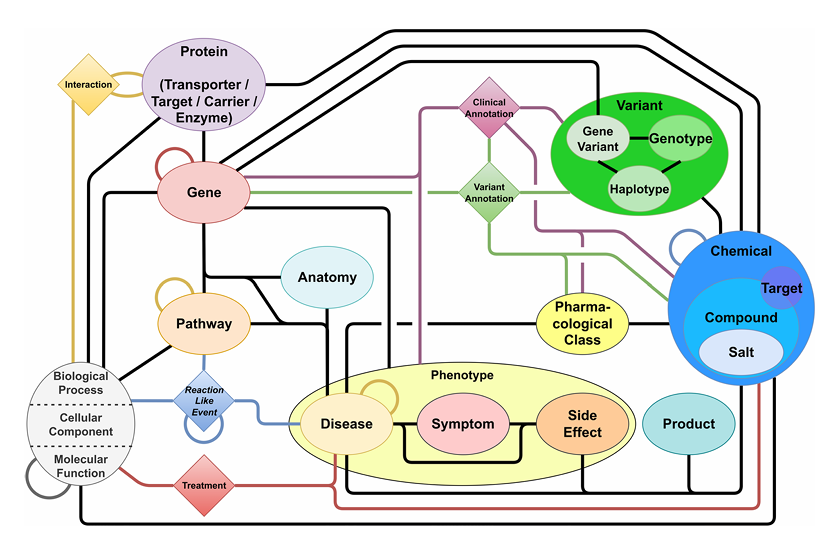
\includegraphics[width=0.75\linewidth]{figures/kg_schema.png}
    \caption{Schema del KG PharMeBiNet \cite{konig}.}
    \label{fig:kg_schema}
\end{figure}


\subsection{Analisi esplorativa del dataset}
Prima di procedere con la sperimentazione, il grafo è stato sottoposto a un'analisi esplorativa sistematica volta a caratterizzarne la struttura topologica e a identificare il sottografo tematico più adatto al task di link prediction. L'analisi ha rivelato una forte eterogeneità nella distribuzione dei nodi e delle relazioni: le entità più numerose sono le varianti genomiche, seguite dai composti chimici e dalle malattie, mentre la distribuzione dei gradi risulta fortemente asimmetrica, con alcuni nodi che raggiungono decine di migliaia di connessioni.
Questa caratteristica ha implicazioni dirette sulla scelta degli algoritmi: modelli che aggregano indiscriminatamente l'intero vicinato risultano computazionalmente intrattabili su nodi ad alto grado, rendendo necessario un meccanismo di campionamento, come quello adottato da GraphSAGE, oppure un approccio che non richieda aggregazione di vicinato, come TransE. I
risultati dettagliati dell'analisi esplorativa, comprensivi delle query Cypher e delle distribuzioni statistiche, sono riportati nel capitolo dei risultati.
\end{comment}

\section{Strumenti e tecnologie}
L'implementazione della pipeline sperimentale si basa su un insieme di strumenti complementari, ciascuno selezionato per soddisfare requisiti specifici del flusso di elaborazione.

\subsection{Neo4j Enterprise}
Neo4j è il Graph DBMS adottato per la gestione del Knowledge Graph PharMeBiNet. La sua architettura nativa a Property Graph garantisce attraversamenti in tempo costante $O(1)$ per ogni passo di traversata, indipendentemente dalla dimensione complessiva del database. La versione Enterprise è stata scelta per la sua capacità di operare in configurazione cluster con topologia primary-secondary, che consente di valutare l'impatto della scalabilità orizzontale sulle prestazioni di lettura. 

Il linguaggio Cypher, nativamente orientato all'attraversamento di percorsi su grafi, permette di esprimere in modo intuitivo le query di estrazione dei sottografi.

\subsection{Libreria Graph Data Science}
La libreria GDS estende Neo4j con implementazioni parallele di algoritmi analitici su grafi, esposti come procedure Cypher. Il suo meccanismo centrale è la \textbf{graph projection}: prima dell'esecuzione di un algoritmo, il sottografo di interesse viene proiettato in una struttura in memoria separata, denominata \textit{graph catalog}, ottimizzata per il calcolo analitico. Questa proiezione crea una snapshot isolata del grafo, consentendo l'esecuzione di algoritmi intensivi in parallelo senza lock sul database transazionale. Il graph catalog supporta operazioni di filtro e trasformazione delle proprietà dei nodi e degli archi direttamente in fase di caricamento, riducendo il pre-processing necessario nella pipeline di machine learning. Questo separa nettamente il layer transazionale da quello analitico, permettendo l'esecuzione di algoritmi intensivi senza interferire con le operazioni correnti sul database e garantendo al contempo che le proiezioni possano essere riutilizzate per molteplici algoritmi senza ripetere il caricamento.

\begin{figure}[ht!]
\centering
\resizebox{0.65\textwidth}{!}{
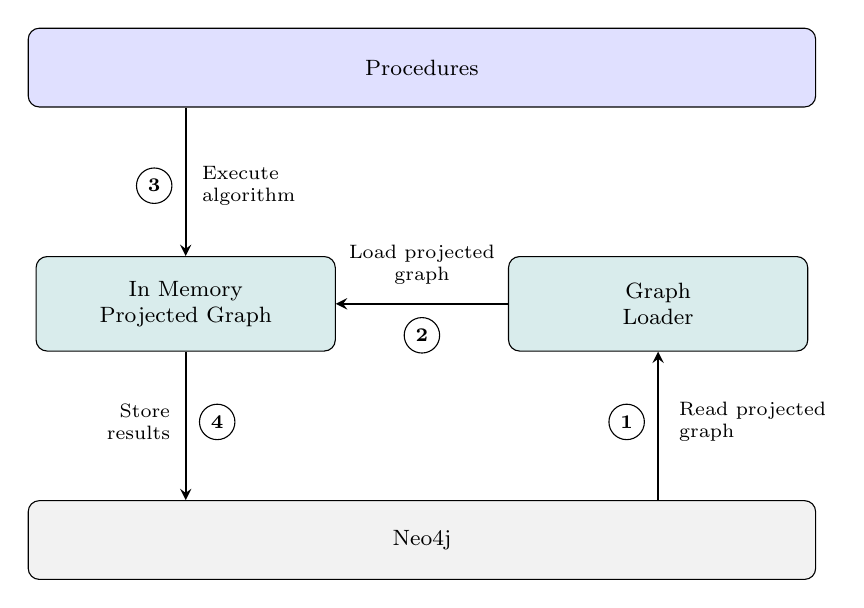
\begin{tikzpicture}[
  box/.style={rectangle, draw, rounded corners, minimum height=1cm,
              font=\footnotesize, align=center},
  wide_box/.style={box, minimum width=10cm},
  node_box/.style={box, minimum width=3.8cm, minimum height=1.2cm},
  arrow/.style={->, thick, >=stealth},
  number/.style={circle, draw, fill=white, inner sep=1.5pt,
                 minimum size=0.45cm, font=\scriptsize\bfseries}
]
  \node[wide_box, fill=blue!12]  (proc)   at (0, 6) {Procedures};
  \node[wide_box, fill=gray!10]  (neo4j)  at (0, 0) {Neo4j};
  \node[node_box, fill=teal!15]  (impg)   at (-3, 3)
    {In Memory\\Projected Graph};
  \node[node_box, fill=teal!15]  (loader) at (3, 3)
    {Graph\\Loader};

  \draw[arrow] (neo4j.north -| loader.south) -- (loader.south);
  \node[align=left, font=\scriptsize] at (4.2, 1.5)
    {Read projected\\graph};
  \node[number] at (2.6, 1.5) {1};

  \draw[arrow] (loader.west) -- (impg.east);
  \node[align=center, font=\scriptsize] at (0, 3.5)
    {Load projected\\graph};
  \node[number] at (0, 2.6) {2};

  \draw[arrow] (proc.south -| impg.north) -- (impg.north);
  \node[align=left, font=\scriptsize] at (-2.2, 4.5)
    {Execute\\algorithm};
  \node[number] at (-3.4, 4.5) {3};

  \draw[arrow] (impg.south) -- (neo4j.north -| impg.south);
  \node[align=right, font=\scriptsize] at (-3.6, 1.5)
    {Store\\results};
  \node[number] at (-2.6, 1.5) {4};
\end{tikzpicture}
}
\caption{Ciclo di vita dell'esecuzione degli algoritmi tramite la libreria Neo4j GDS: il grafo viene proiettato in memoria, l'algoritmo viene eseguito sulla proiezione e i risultati vengono scritti nel database.}
\label{fig:neo4j_gds_architecture}
\end{figure}

\subsection{PyTorch Geometric}
PyTorch Geometric \cite{fey2019fast} è il framework di riferimento per l'implementazione dei tre modelli di Graph Machine Learning. Sviluppato come estensione di PyTorch, fornisce primitive efficienti per la rappresentazione di grafi eterogenei attraverso il formato \texttt{HeteroData}, layer convoluzionali dedicati (come \texttt{SAGEConv}) e utility per la suddivisione del dataset in training, validazione e test. Il supporto nativo al calcolo tensoriale su GPU e la possibilità di definire meccanismi di message passing personalizzati lo rendono particolarmente adatto per sperimentare con architetture diverse su grafi di larga scala.

\subsection{Containerizzazione e automazione infrastrutturale}
L'ambiente Neo4j su ciascun nodo del cluster è containerizzato tramite \textbf{Docker}, garantendo isolamento delle dipendenze e riproducibilità dell'esecuzione indipendentemente dal sistema operativo sottostante. \textbf{Docker Compose} coordina la definizione e l'avvio dei servizi tramite un unico file YAML, semplificando il deployment e la gestione delle versioni del database.

La gestione orchestrata del cluster è affidata ad \textbf{Ansible}, che tramite playbook dichiarativi eseguiti via SSH consente di distribuire configurazioni, avviare e fermare i container, sincronizzare file tra i nodi ed eseguire il benchmark nelle diverse configurazioni con un singolo comando. L'assenza di agenti e l'uso di un linguaggio YAML leggibile garantiscono riproducibilità e coerenza tra gli ambienti.

Le quattro macchine virtuali che costituiscono il cluster sono ospitate su \textbf{Microsoft Azure}, ciascuna con 8 core virtuali e 32 GB di RAM, all'interno di una stessa rete virtuale per garantire bassa latenza nelle comunicazioni intra-cluster. La scelta di Azure consente di sfruttare la scalabilità elastica e la possibilità di replicare l'infrastruttura in diverse regioni per futuri esperimenti.

I dettagli implementativi della configurazione, inclusi i comandi di deployment, le impostazioni di memoria e la gestione degli indirizzi IP su WSL2, sono riportati nel capitolo di Implementazione (Sezione \ref{sec:implementation}).

\section{Il dataset: PharMeBiNet V3}

\textbf{PharMeBiNet} (\textit{Pharmacological Medical Biochemical Network}) è un knowledge graph biomedico open-source \cite{konigs2022pharmebinet} che integra informazioni provenienti da oltre quaranta sorgenti farmacologiche, genomiche e cliniche, tra cui DrugBank, ClinVar, CTD, DisGeNET e UniProt. Il progetto nasce come estensione di Hetionet e ne estende la copertura semantica con ulteriori tipi di entità e relazioni.

La versione \textbf{V3} \cite{pharmebinet_zenodo} è quella adottata in questo lavoro. Come illustrato in Figura \ref{fig:kg_schema}, il grafo modella un'ampia varietà di entità biologiche come: farmaci, geni, proteine, malattie, varianti genomiche e reazioni avverse e le relazioni che le interconnettono, quali interazioni farmaco-farmaco, associazioni gene-malattia e percorsi metabolici.

\begin{figure}[ht!]
    \centering
    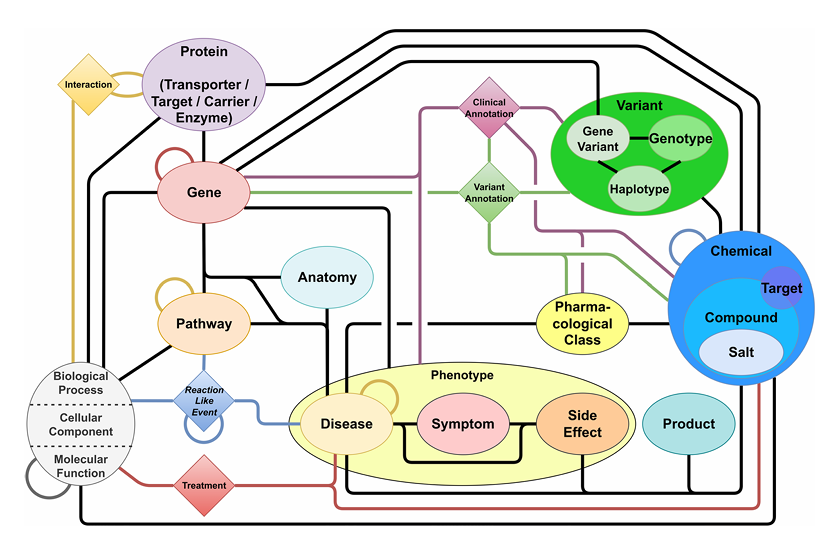
\includegraphics[width=0.80\linewidth]{figures/kg_schema.png}
    \caption{Schema del KG PharMeBiNet \cite{konig}.}
    \label{fig:kg_schema}
\end{figure}